\documentclass{article}
\usepackage[utf8]{inputenc}
\usepackage{fancyhdr}
\usepackage{graphicx}
\usepackage{float}
\usepackage{geometry}
\usepackage[font=small,labelfont=bf]{caption}
\usepackage{caption}
\captionsetup[figure]{font=small}
\usepackage[justification=centering]{caption}
\usepackage{courier}

% ---- Commands ------- %
\newcommand{\documentNumber}[1]{
    \LARGE  \textbf{ PUSS21420{#4} } \\
    \medskip
}
\newcommand{\documentVersion}[1]{
    v. {#1}

    \medskip
}
\newcommand{\documentTitle}[1]{
    \centerline{\rule{13cm}{0.4pt}}
    \bigskip \bigskip
    \LARGE \textbf{TimeMate} \\
    \bigskip
    \LARGE {#1} \\
    \bigskip \bigskip
    \centerline{\rule{13cm}{0.4pt}}
}
\newcommand{\documentGroup}[1]{
    \bigskip \bigskip
    \LARGE Group {#1} \\
    \bigskip
}
\newcommand{\documentResponsible}[1]{
    \LARGE Responsible: {#1} \\
    \medskip
}
\newcommand{\documentAuthors}[1]{
    \LARGE Authors: {#1} \\
    \medskip    
}
\newcommand{\documentDate}[1]{
    \date {#1} 
}

\graphicspath{{./images/}} % Defines a path to file images
\renewcommand{\arraystretch}{1.7}  % Vertical padding for tables


% --- Header & Footer ---- %
\pagestyle{fancy}
\lhead{\leftmark}
\rhead{}
\rfoot{\thepage}
\cfoot{}
\lfoot{}


% ------------------------------------------------ #

% ----- FILL THIS ----- %
\title {
    % Must be 2 digits
    \documentNumber {01}    
    
    % BASELINE.VERSION
    \documentVersion {0.1}
    
    % Full name - SHORTNAME
    \documentTitle {Software Top Level Design Document}
    \documentGroup {2}
    
    % Options: - Project Management Group
    %          - System Architecture Group
    %          - Developer Group
    %          - Test Group
    \documentResponsible {System Group}
    \documentAuthors {Developer Group}
    
    % Format: YYYY-MM-DD
    \documentDate {2021-02-11}
}

\begin{document}

\maketitle
\thispagestyle{empty}

\newpage

\tableofcontents

\newpage

%---------Document begins here-----------

% FILL IN CORRECT VERSION HISTORY!
% Not sure? Refer to SDP how it works or ask someone!
\section{Document History}
\begin{tabular}{ l | l | l | l }
    Version & Date & Responsible & Description \\
    \hline
    0.1 & 2021-02-11 & UG & Document created. \\
\end{tabular}

\section{Introduction}
This document describes the design of "TimeMate". The system is a further development of the system "BaseBlockSystem". "TimeMate" hosts various functions related to the creating of time reports, getting a view of reported time and more.

\section{Reference Documents}
\begin{enumerate}
    \item Software Requirements Specification: TimeMate, v. 0.5, Doc. number: PUSS214201
    \item Software Top Level Design Document: BaseBlockSystem, v 1.0, Doc. number: PUSS12004
\end{enumerate}

\section{Terminology}
\begin{itemize}
\item \textbf{Java Server Page (JSP):} Server-side technology that enables the creation of dynamic views.
\item \textbf{Servlets:} Java programs that run on the server side.
\item \textbf{Java Beans:} A Java class that only contains set/get methods with private attributes.
\end{itemize}

\section{Overview}
Placeholder for the overview of the project - replace with information regarding the project.

\subsection{Java Server Pages}
Below are the pages used for "TimeMate" and what their function is.

\subsubsection{login.jsp}
The view that is shown when a user that is not logged tries to access the system. This is the only page in the "TimeMate" system a user can get access to without having an account. The page consists of two fields,  one for username and one for password, as well as an option to request a new password in case the user has forgotten their password.  If the user chooses to reset their password, a pop up is shown where the user can enter their e-mail which the new password will be sent to.

\subsubsection{index.jsp}
This file contains the view that is shown when a user has logged in. From here,  the user can access the menu which is dynamically updated depending on what group the user belong to. The index page contains overview information about TimeMate.

\subsubsection{viewReport.jsp}
This file contains the view that shows a collection of the users submitted reports. When being here, the user can select a submitted report to show more information about.

\subsubsection{newReport.jsp}
This file contains the view that represents the creation of a new time report.

\subsubsection{editReport.jsp}
This view is used by users that want to edit their previously reported time reports. When being here, the user can select a submitted report to edit.

\subsubsection{summaryReport.jsp}
This view represents a summary of a user's previously reported time reports.

\subsubsection{signReport.jsp}
This view is used by the project leaders for signing and unsigning time reports.

\subsubsection{usermanagement.jsp}
This file contains the view of the usermanagement page. The view is used by the administrator and the project leaders.

\subsubsection{administration.jsp}
This file contains the view of the administration page. Only the administrator has access to this view.

\subsubsection{changepassword.jsp}
This view is used by all users to change their password. The page contains three fields, one for the user's current password, and two for the new password (in order to confirm it).

\subsection{Servlets}
The files below are the controllers for the system.

\subsubsection{LoginServlet}
Communication link between the view login.jsp and the bean LoginBean.

\subsubsection{PasswordChangerServlet}
Servlet used when a user changes their password.

\subsubsection{TimeReportServlet}
Communication link between the views viewReport.jsp, newReport.jsp and summaryReport.jsp and the bean ReportBean.

\subsubsection{TimeReportManagementServlet}
Communication link between the views editReport.jsp and signReport.jsp and the bean ReportBean

\subsubsection{UserManagementServlet}
Communication link between the view usermanagement.jsp and the bean UserManagementBean.

\subsubsection{AdministrationServlet}
Communication link between the view administration.jsp and the bean AdministrationBean.

\subsection{Java Beans}
The files below are the Java Beans that are used to send information from the server to the client view. When created, beans are stored in the current session and discarded when the session ends.

\subsubsection{UserBean}
Get/set class which contains user information required to execute queries and updates related to the logged in user.

\subsubsection{TimeReportBean}
Get/set class which contains a list of users and their time reports which is required to render the report.jsp view.

\subsubsection{UserManagementBean}
Get/set class which contains a list of users(Excluding project leaders) and their roles which is required to render the usermanagement.jsp view.

\subsubsection{AdministrationBean}
Get/set class which contains a list of users and their roles (Including project leaders) which is required to render the administration.jsp view.

\subsection{Other classes}
The classes below are never accessed by the user in any way, but are instead helper classes to the servlets.

\subsubsection{MailHandler}
Class used to send e-mails to users upon account creation and password changes.

\subsubsection{PasswordHandler}
Class used to encrypt passwords when needed.

\subsubsection{Database}
Class to establish connection between Tomcat and the database.

\section{Database}
In this project, there is one database that consists of the nine relations shown in Figure 1. Every relation has one primary key each, which are the following: \emph{userID}, \emph{projectID} and \emph{reportID}.

\begin{figure}[h]
     \centering
     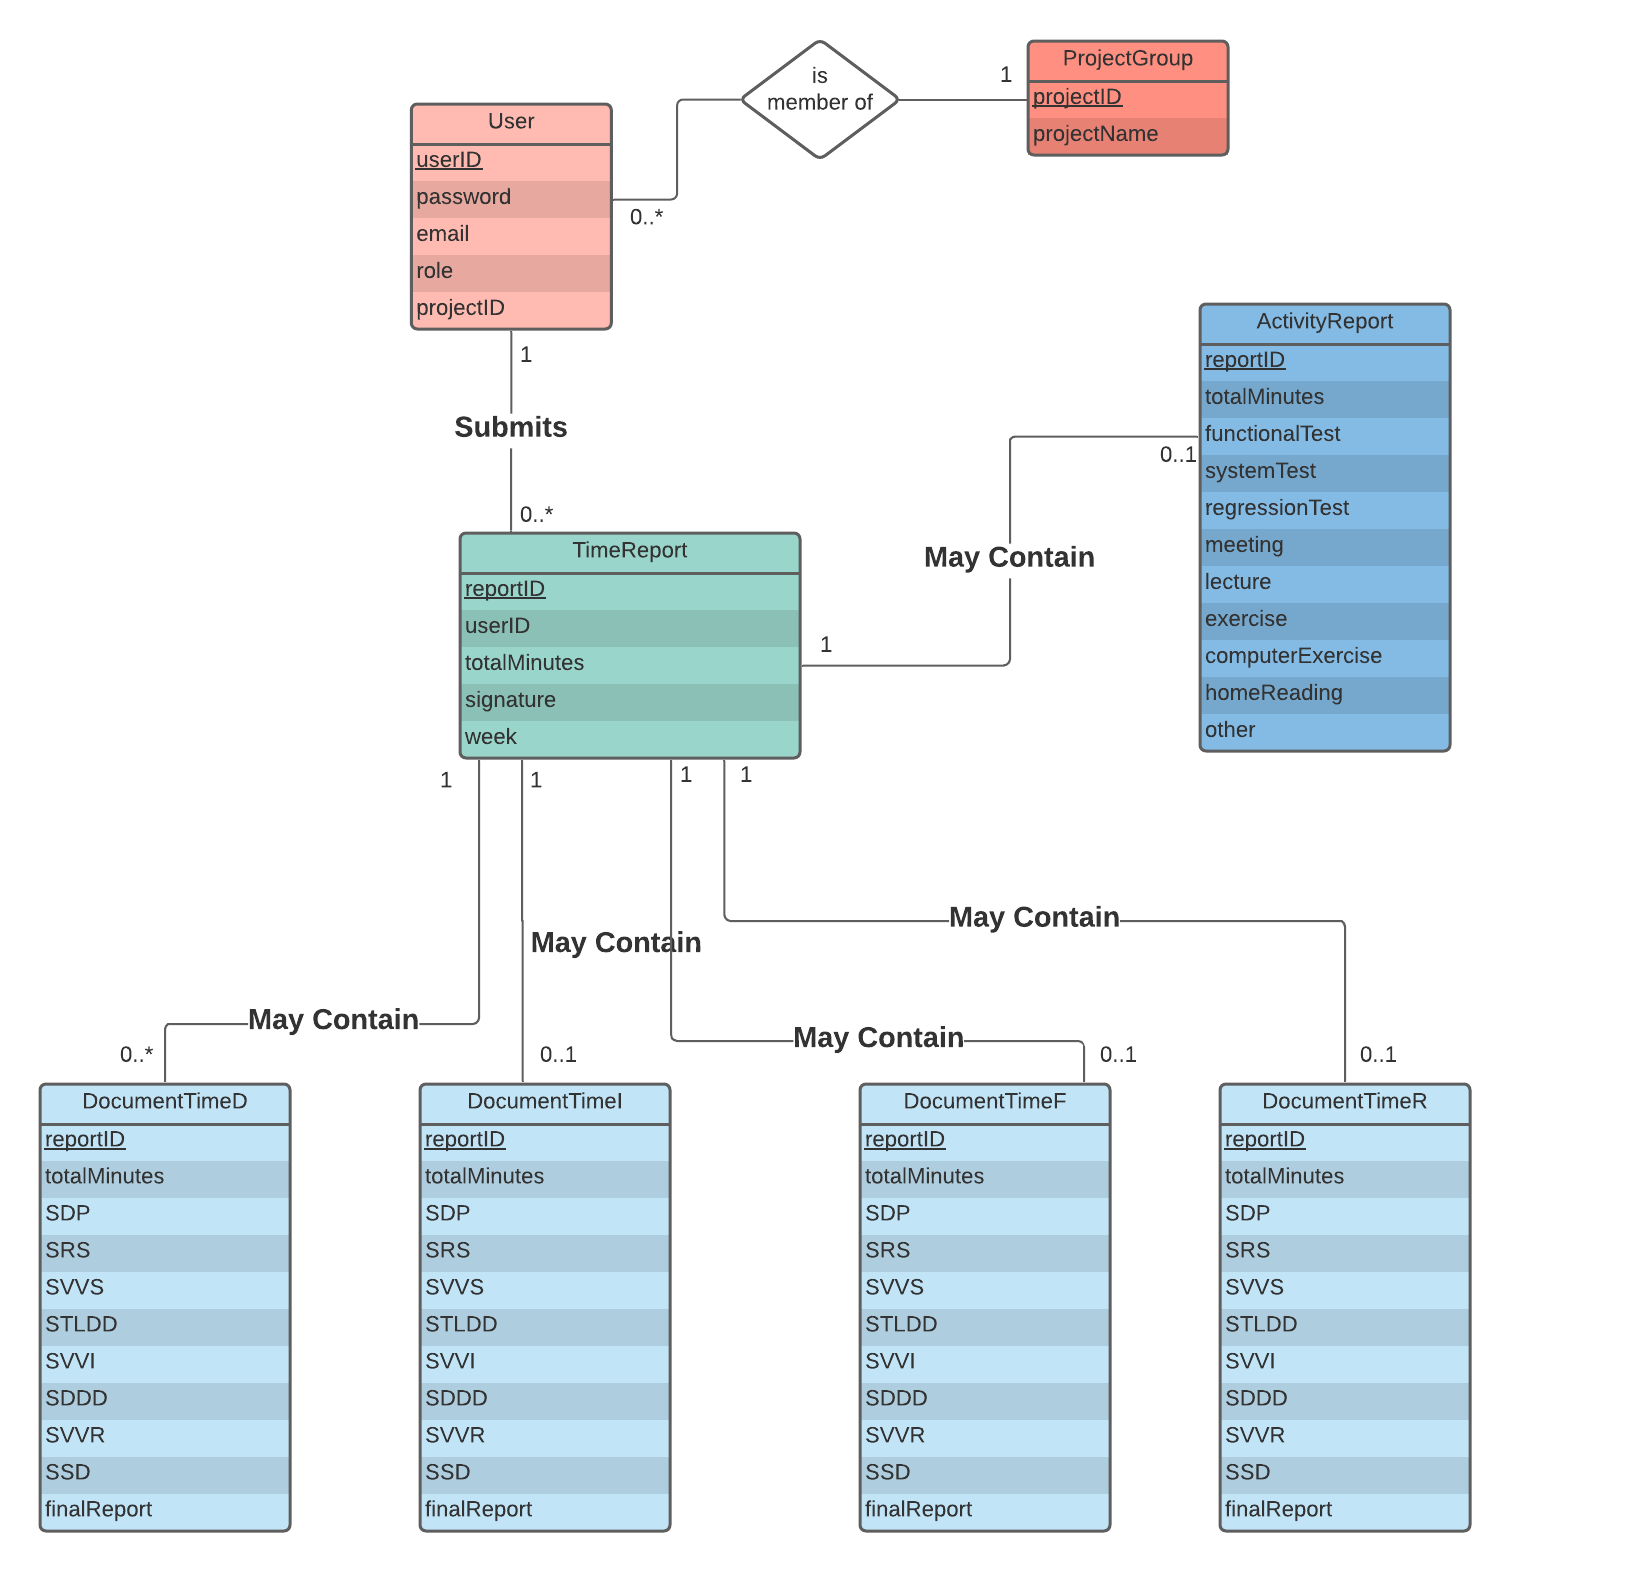
\includegraphics[width=10cm]{images/PUSPERdiagramVers3.png}
     \renewcommand\figurename{Figure}
     \caption{The database consists of the following relations: \emph{User}, \emph{ProjectGroup}, \emph{TimeReport}, \emph{ActivityReport} and \emph{DocumentTimeD/I/F/R}. \emph{Is member of} represents the relationship between User and ProjectGroup.}
     \label{fig:my_label}
 \end{figure}

\subsection{User Relation}
The User relation contains all registered users together with user specific information such as password, email and information about whether a user belongs to a project group or not. A user belonging to a group may be assigned a role under the role attribute. The username attribute is used as the primary key, making every username unique. A User table can be created using the following MySQL command:
\newline

\small
\texttt{
\noindent mysql> CREATE TABLE User (\newline
\indent\indent\indent -> userID Integer NOT NULL,\newline
\indent\indent\indent -> password varChar(50) NOT NULL,\newline
\indent\indent\indent -> email varChar(100),\newline
\indent\indent\indent -> role varChar(30),\newline
\indent\indent\indent -> projectID Integer,\newline
\indent\indent\indent -> PRIMARY KEY(userID),\newline
\indent\indent\indent -> FOREIGN KEY(projectID) REFERENCES ProjectGroup(projectID)\newline
\indent\indent\indent -> ON UPDATE CASCADE ON DELETE SET NULL\newline
\indent\indent\indent -> );\newline
}
\normalsize

\subsection{ProjectGroup Relation}
The ProjectGroup relation contains all project group IDs and connects an ID to a project name. The projectID attribute is used as the primary key, enabling two or more project groups to be registered under the same name but still be distinguished from one another by their IDs.
\newline

\small
\texttt{
\noindent mysql> CREATE TABLE ProjectGroup (\newline
\indent\indent\indent -> projectID Integer NOT NULL,\newline
\indent\indent\indent -> projectName varChar(30) NOT NULL,\newline
\indent\indent\indent -> PRIMARY KEY(projectID)\newline
\indent\indent\indent -> );
}
\normalsize

\subsection{TimeReport Relation}
The time report to be filled out by each individual user on a weekly basis contains 55 columns, aiming to help the user specify the time spent on various activities. Four sections - \emph{D (Development)}, \emph{I (Informal review)}, \emph{F (Formal review)}, \emph{R (Rework, improvement or correction)}. However, there may be weeks where no time is spent on, e.g.,  formal reviews. In that case, a large number of columns would be wasted, as there will be no meaningful data added to the columns related to that section of the time report. 
\newline

\small
\texttt{
\noindent mysql> CREATE TABLE TimeReports (\newline
\indent \indent \indent -> reportID Integer NOT NULL,\newline
\indent \indent \indent -> userID Integer NOT NULL,\newline
\indent \indent \indent -> totalMinutes Integer,\newline
\indent \indent \indent -> signature Integer,\newline
\indent \indent \indent -> week Integer NOT NULL,\newline
\indent \indent \indent -> PRIMARY KEY(reportID),\newline
\indent \indent \indent -> FOREIGN KEY(userID) REFERENCES User(userID)\newline
\indent \indent \indent -> ON UPDATE CASCADE ON DELETE CASCADE\newline
\indent \indent \indent -> FOREIGN KEY(signature) REFERENCES User(userID)\newline
\indent \indent \indent -> ON UPDATE CASCADE ON DELETE SET NULL\newline
\indent \indent \indent -> );
}
\normalsize
\newline

To avoid data redundancy, the time reports are being separated into several different relations. The reason for this is the fact that every single submitted time report is going to be represented in TimeReports: (here we can include the relation)

\subsection{ActivityReport Relation}
ActivityReport is the relation concerning the general activity types. As can be seen in Figure 1, these include the unique primary key: reportID and other attributes such as homeReading, meeting and various tests.
\newline

\small
\texttt{
\noindent mysql> CREATE TABLE ActivityReport (\newline
\indent\indent\indent -> reportID Integer NOT NULL,\newline
\indent\indent\indent -> totalMinutes Integer,\newline
\indent\indent\indent -> functionalTest Integer,\newline
\indent\indent\indent -> systemTest Integer,\newline
\indent\indent\indent -> regressionTest Integer,\newline
\indent\indent\indent -> meeting Integer,\newline
\indent\indent\indent -> lecture Integer,\newline
\indent\indent\indent -> exercise Integer,\newline
\indent\indent\indent -> computerExercise Integer,\newline
\indent\indent\indent -> homeReading Integer,\newline
\indent\indent\indent -> other Integer,\newline
\indent\indent\indent -> PRIMARY KEY(reportID),\newline
\indent\indent\indent -> FOREIGN KEY(reportID) REFERENCES TimeReport(reportID)\newline
\indent\indent\indent -> ON UPDATE CASCADE ON DELETE CASCADE\newline
\indent\indent\indent -> );\newline
}
\normalsize


\subsection{DocumentTimeD/I/F/R Relation}
As mentioned earlier, there are four different activity types in the time documentation: \emph{Development and documentation (D)}, \emph{Informal review (I)}, \emph{Formal review (F)} and \emph{Rework, improvement or correction (R)}. All of these relations contain the same attributes mainly concerning the various documents. Besides these attributes, there is one attribute concerning the totalMinutes. The purpose of this attribute is to oversee the amount of minutes spent on each activity type. Since each document continuously is in a different stage, it was concluded to include different phases as activity types to ensure that the time reports are comprehensible. All of these tables can be created by using the same SQL statement:
\newline

\small
\texttt{
\noindent mysql> CREATE TABLE TimeDevelopments (\newline
\indent\indent\indent -> reportID Integer NOT NULL,\newline
\indent\indent\indent -> totalMinutes Integer,\newline
\indent\indent\indent -> SDP Integer,\newline
\indent\indent\indent -> SRS Integer,\newline
\indent\indent\indent -> SVVS Integer,\newline
\indent\indent\indent -> STLDD Integer,\newline
\indent\indent\indent -> SVVI Integer,\newline
\indent\indent\indent -> SDDD Integer,\newline
\indent\indent\indent -> SVVR Integer,\newline
\indent\indent\indent -> SSD Integer,\newline
\indent\indent\indent -> finalReport Integer\newline
\indent\indent\indent -> PRIMARY KEY(reportID),\newline
\indent\indent\indent -> FOREIGN KEY(reportID) REFERENCES TimeReport(reportID)\newline
\indent\indent\indent -> ON UPDATE CASCADE ON DELETE CASCADE\newline
\indent\indent\indent -> );\newline
}
\normalsize

\section{Information Stored in Sessions}

%-Slå ihop 0, 1, 2 eftersom de har samma privileges?
\textbf{Integer CURRENT\textunderscore ROLE:} Used to determine the current users privileges. The following states have been defined:
\medskip

\indent \textbf{0:} Privileges for users in the "UG" group.

\indent \textbf{1:} Privileges for users in the "TG" group.

\indent \textbf{2:} Privileges for users in the "SG" group.

\indent \textbf{3:} Project leader privileges.

\indent \textbf{4:} Administrator privileges.

\pagebreak
\section{Sequence Diagrams}
\subsection{LoginServlet}

\begin{figure}[h]
    \centering
    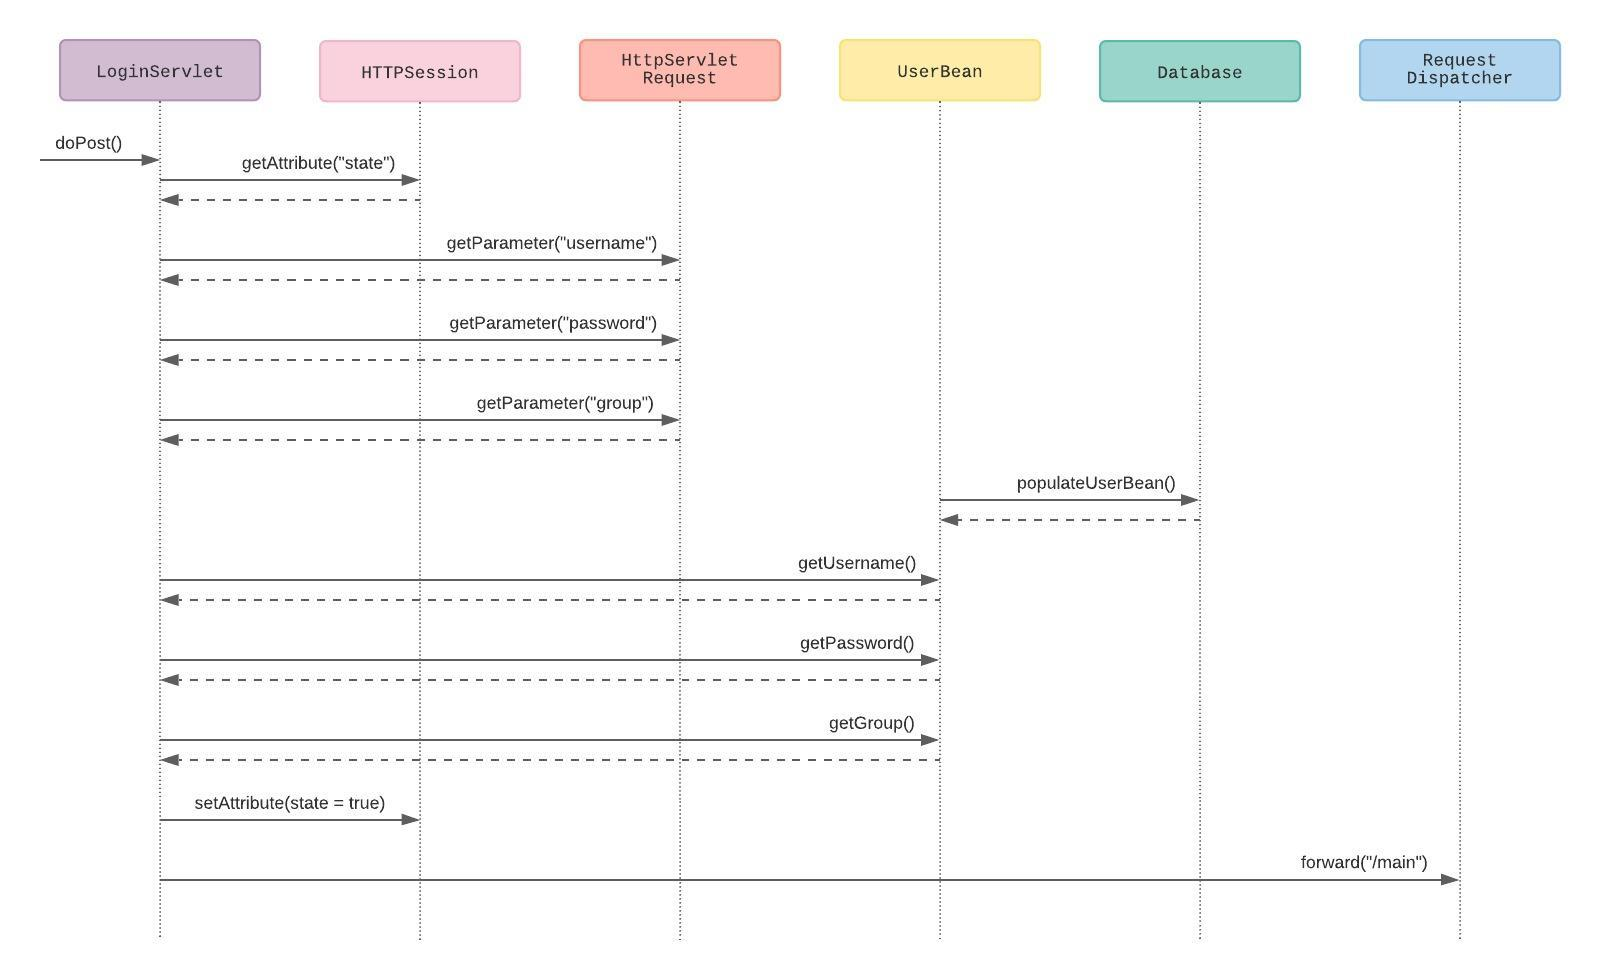
\includegraphics[scale=0.4]{images/successfulLogin.jpeg}
    \caption{Sequence diagram for a successful login.}
    \label{fig:successfulLogin}
\end{figure}

\begin{figure}[h]
    \centering
    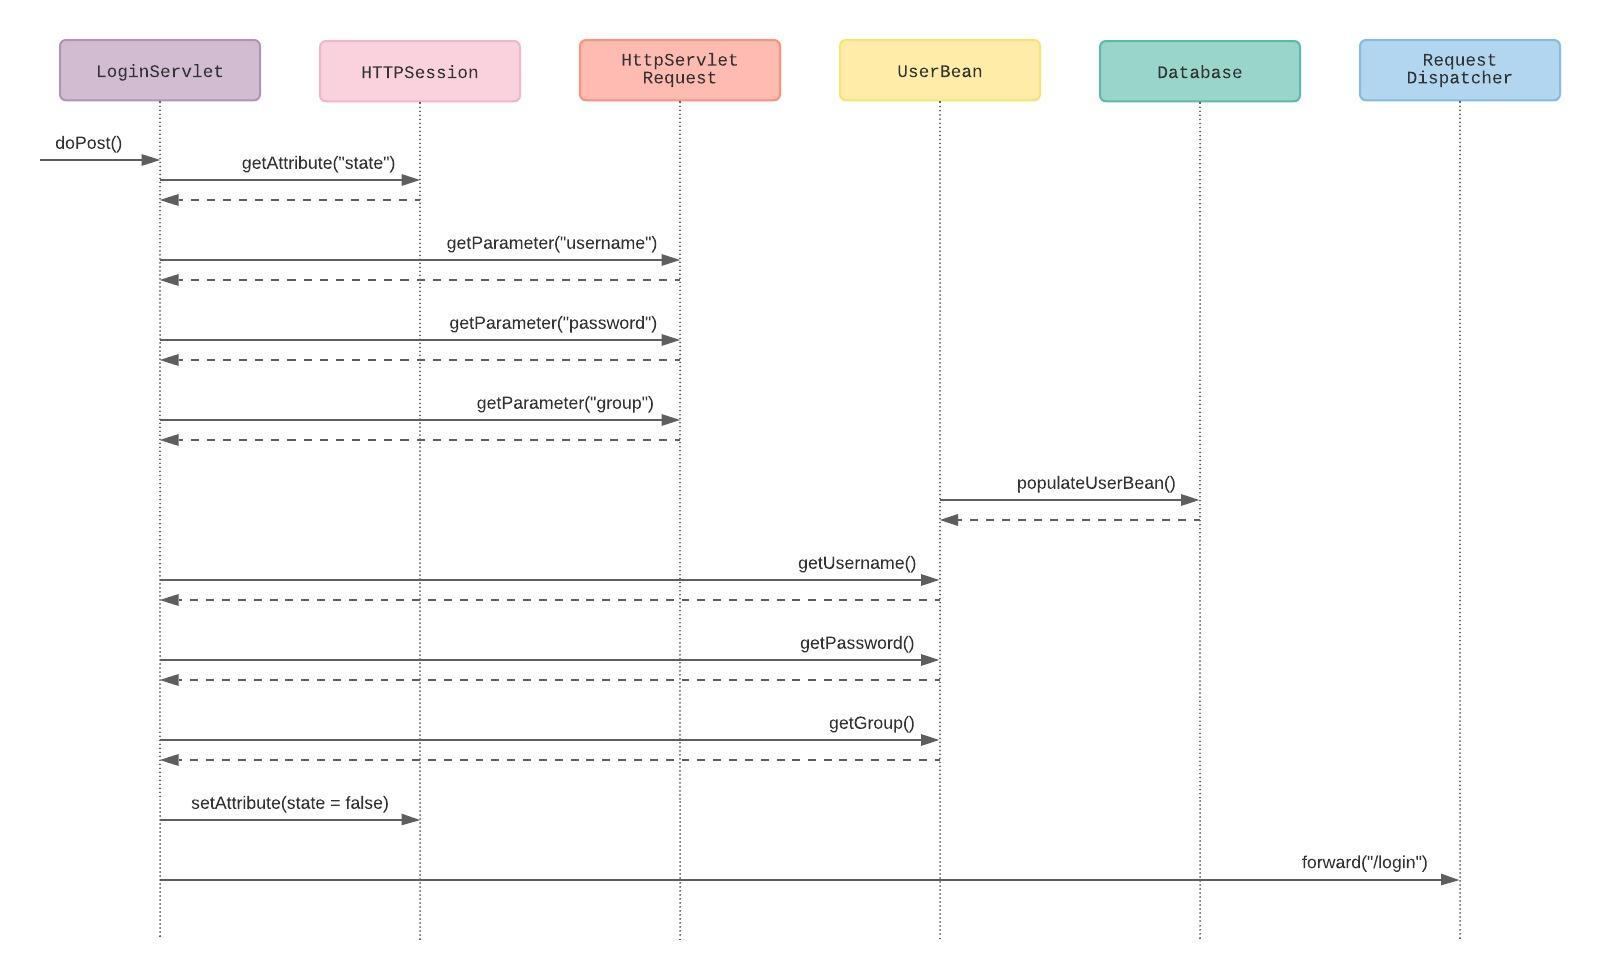
\includegraphics[scale=0.4]{images/failedLogin.jpeg}
    \caption{Sequence diagram for a failed attempt to login.}
    \label{fig:failedLoginAttempt}
\end{figure}

\pagebreak
\subsection{UserManagementServlet}

\begin{figure}[h]
    \centering
    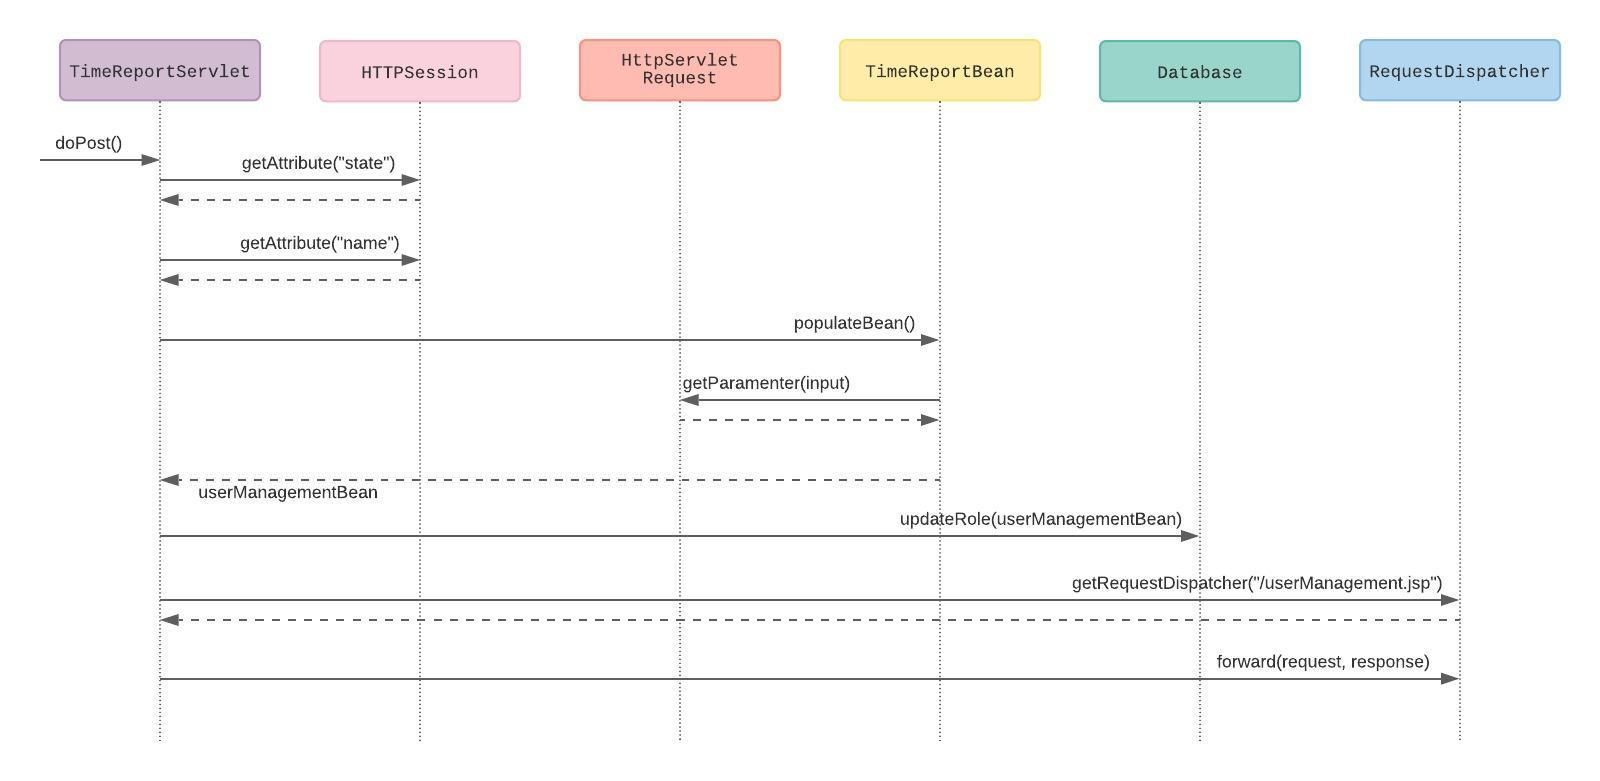
\includegraphics[scale=0.5]{images/updateRole.jpeg}
    \caption{Sequence diagram for the process of updating the role of a project member.}
    \label{fig:successfulLogin}
\end{figure}

\begin{figure}[h]
    \centering
    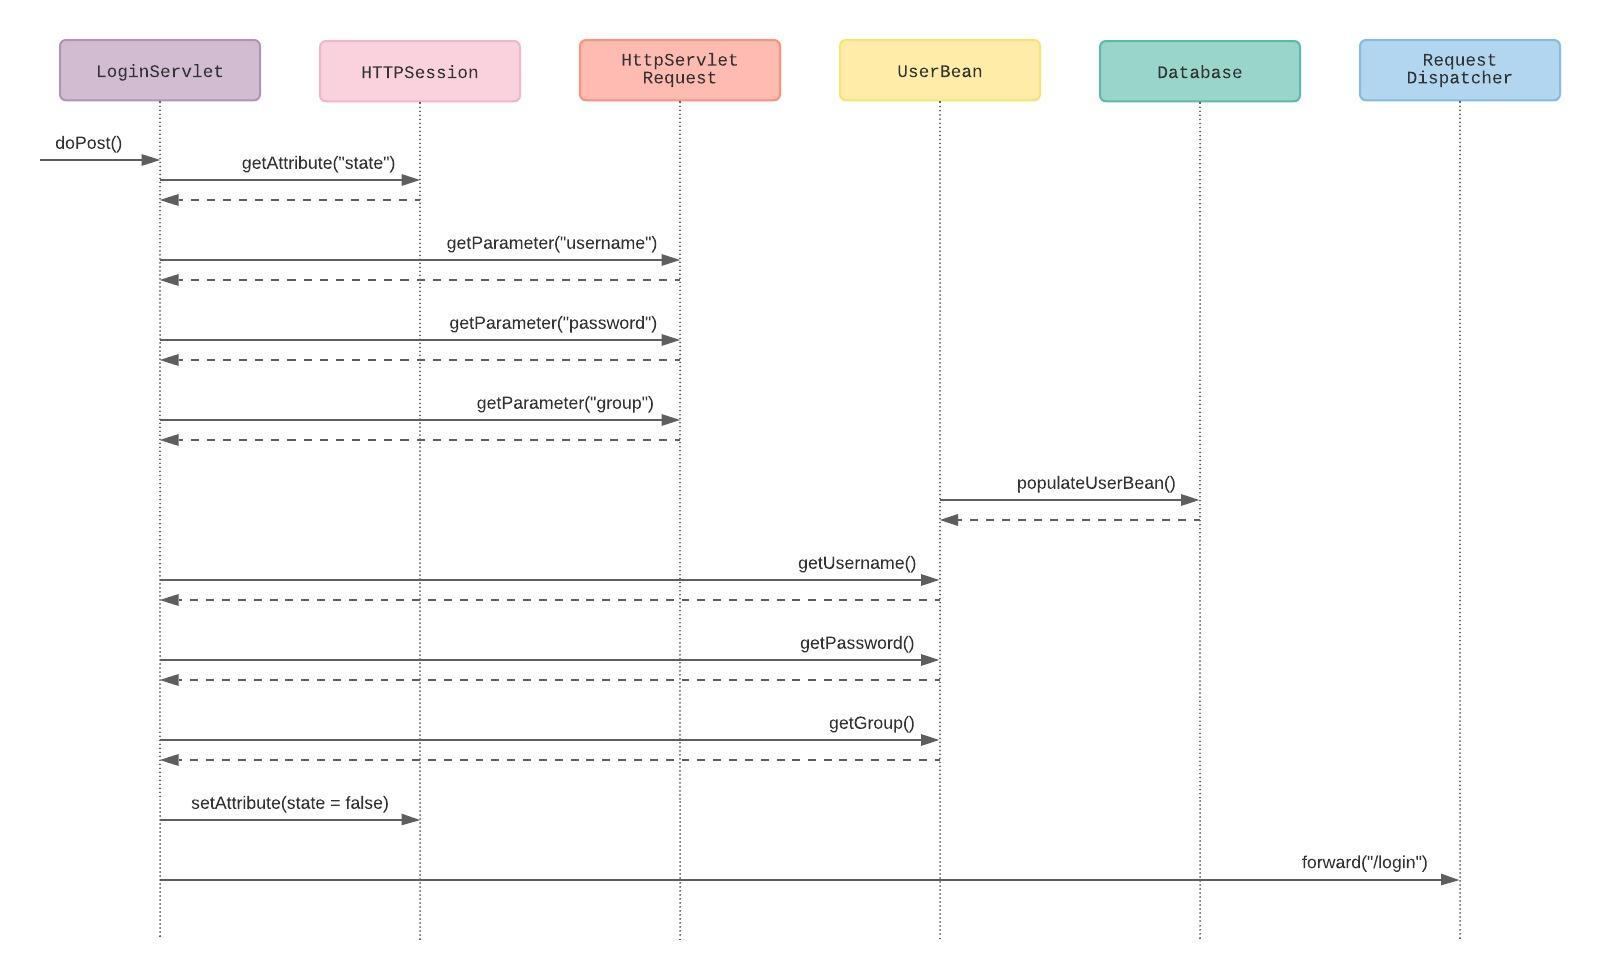
\includegraphics[scale=0.4]{images/failedLogin.jpeg}
    \caption{Sequence diagram for a failed attempt to login.}
    \label{fig:failedLoginAttempt}
\end{figure}

\pagebreak
\subsection{PasswordChangerServlet}

\begin{figure}[h]
    \centering
    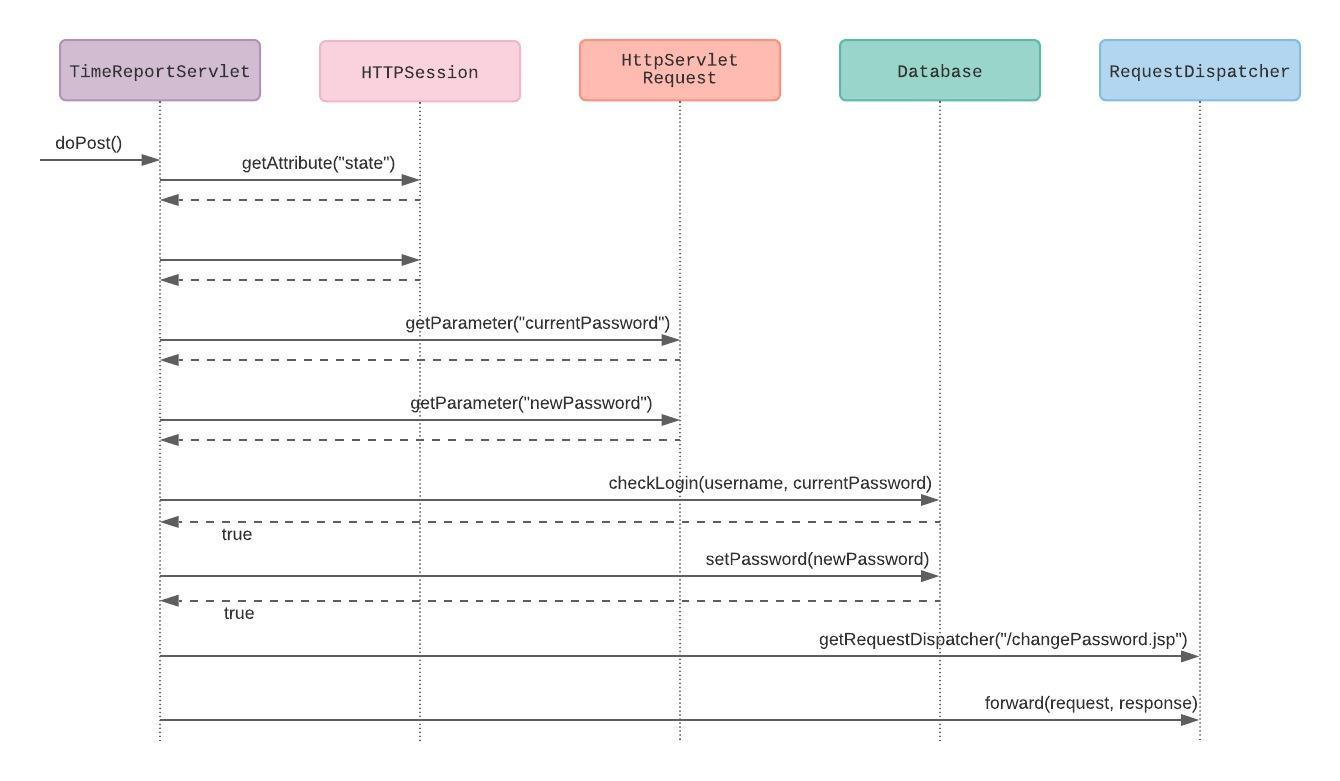
\includegraphics[scale=0.5]{images/successfulPasswordChange.jpeg}
    \caption{A successful password change.}
    \label{fig:sucessfulPasswordChange}
\end{figure}

\begin{figure}[h]
    \centering
    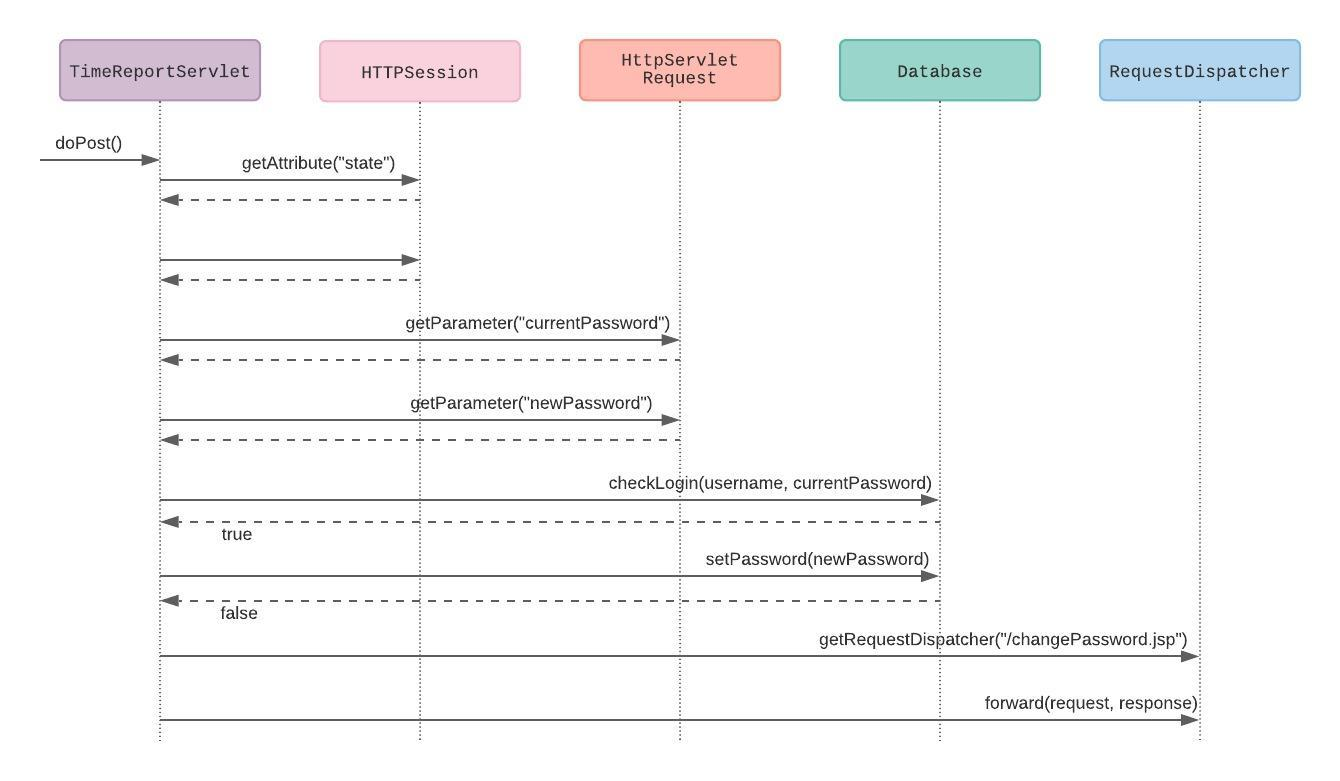
\includegraphics[scale=0.5]{images/unsuccessfulPasswordChange.jpeg}
    \caption{A failed attempt to change password.}
    \label{fig:failedPasswordChange}
\end{figure}

\begin{figure}[h]
    \centering
    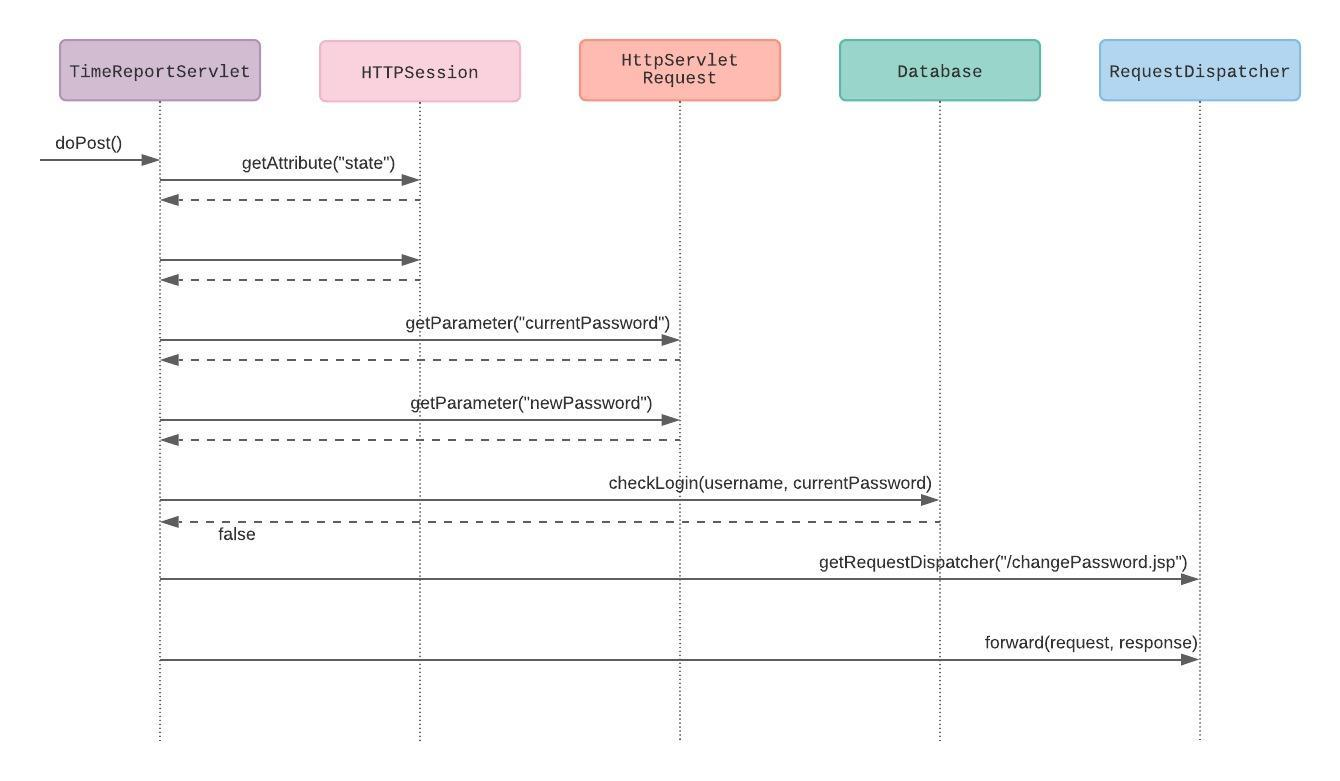
\includegraphics[scale=0.5]{images/changePasswordFalseInput.jpeg}
    \caption{A failed attempt to change password due to incorrect user input.}
    \label{fig:failedPasswordChangeIncorrectInput}
\end{figure}

\pagebreak

\subsection{TimeReportServlet}

\begin{figure}[h]
    \centering
    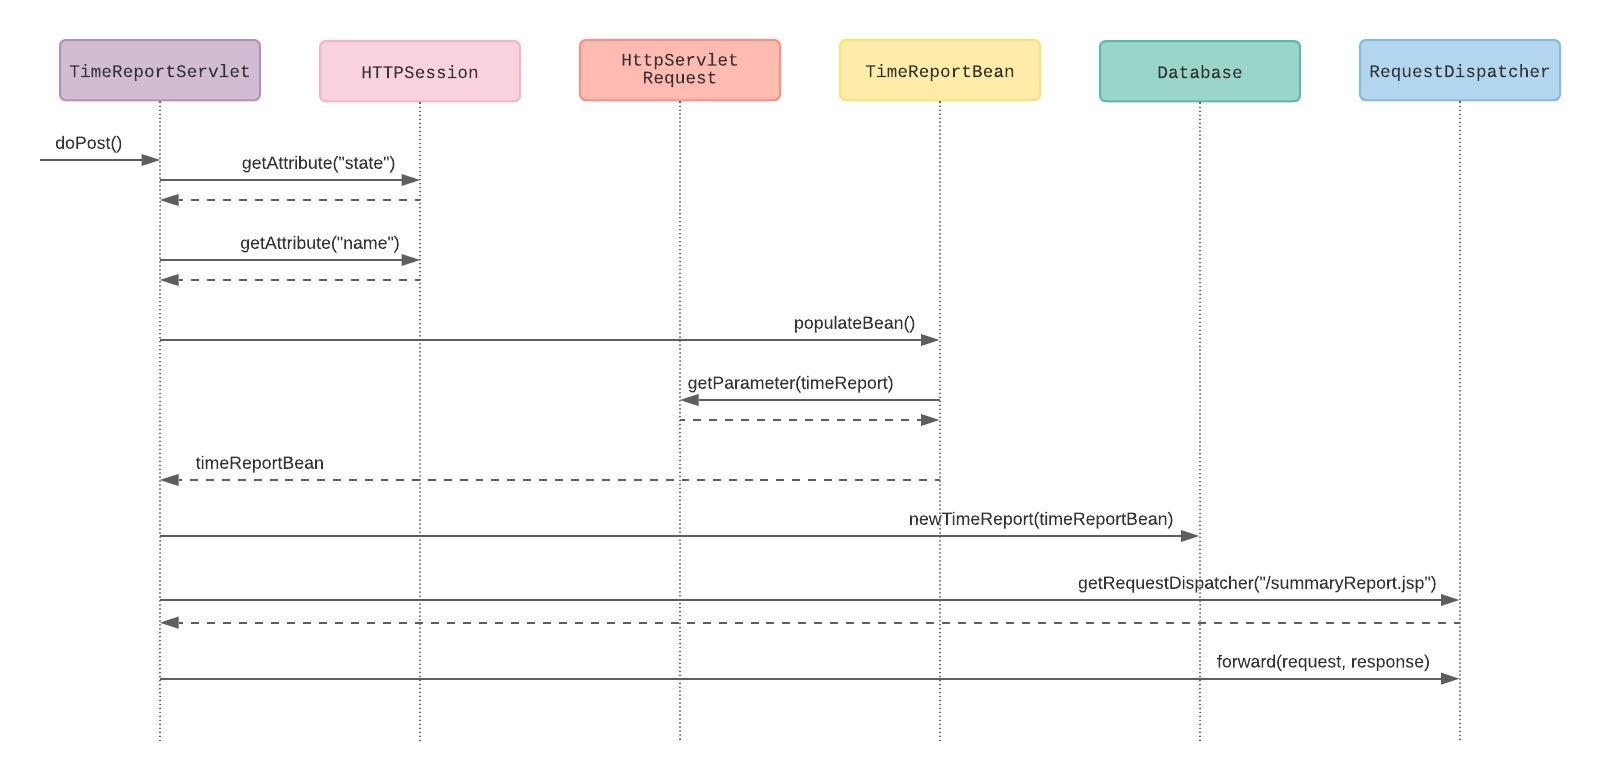
\includegraphics[scale=0.5]{images/addNewTimeReport.jpeg}
    \caption{Adding a new Time Report.}
    \label{fig:newTimeReport}
\end{figure}

\begin{figure}[h]
    \centering
    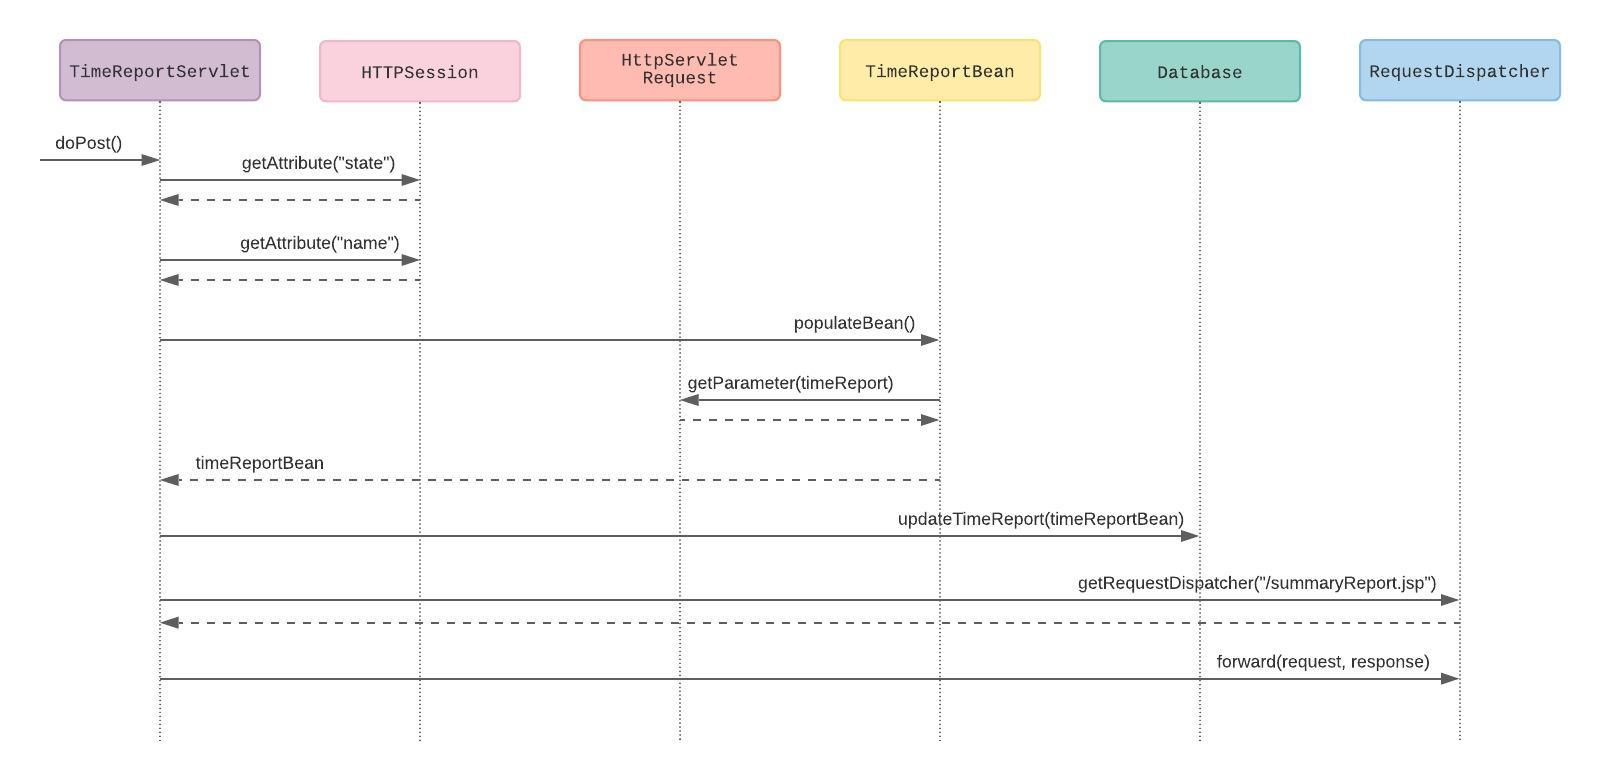
\includegraphics[scale=0.5]{images/editTimeReport.jpeg}
    \caption{Editing a Time Report.}
    \label{fig:editTimeReport}
\end{figure}


\begin{figure}[h]
    \centering
    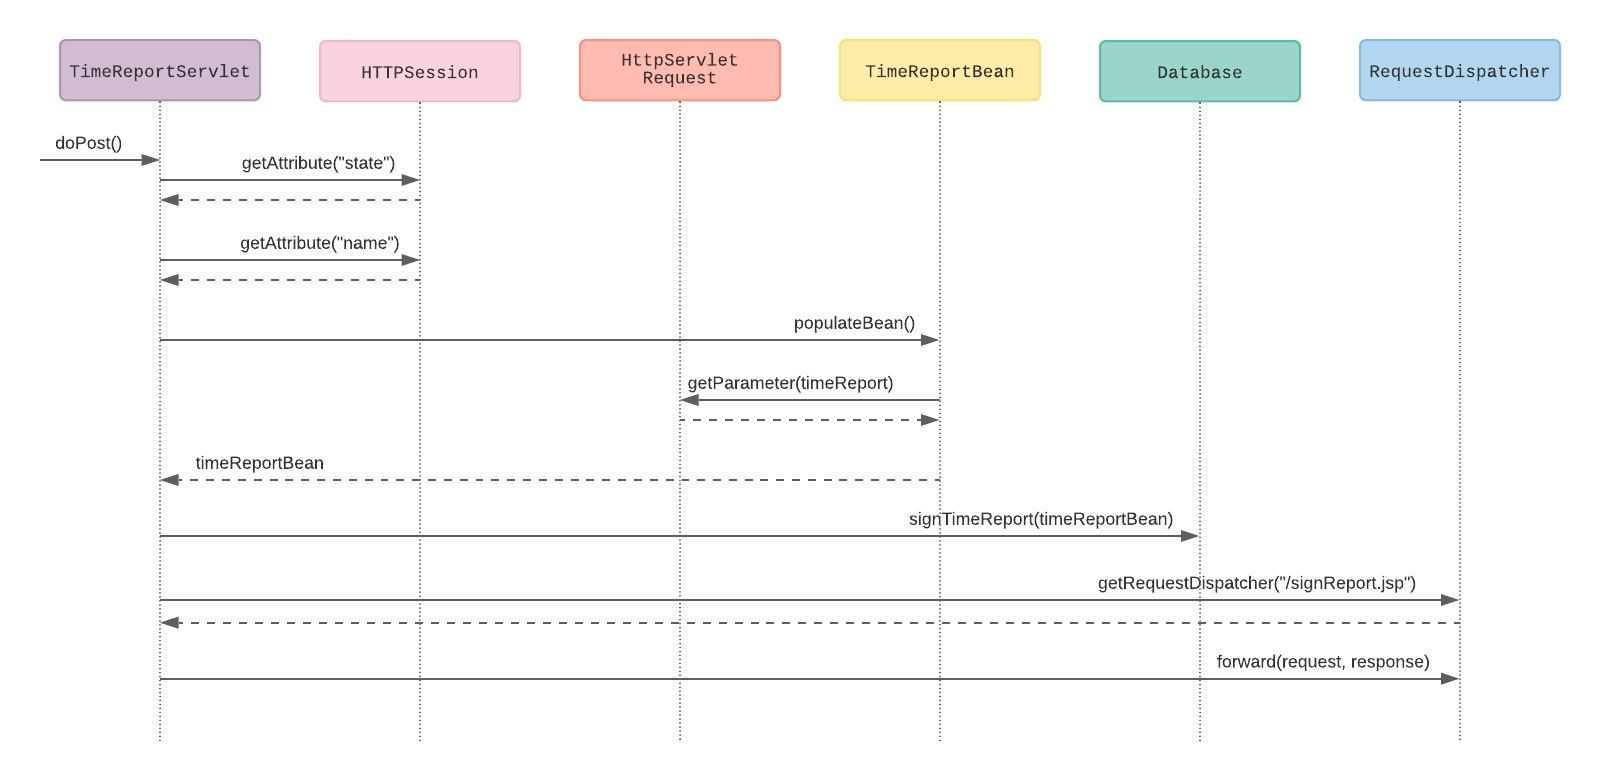
\includegraphics[scale=0.5]{images/signUnsignReports.jpeg}
    \caption{Signing/unsigning a Time Report. This can only be done by the project leader.}
    \label{fig:signunsign}
\end{figure}

\subsection{}

%---------Document ends here-----------

\end{document}